\section{Bilder des Gehäuses}\label{sec_gehaeusebilder}
%
\vspace{5ex}
\centerline{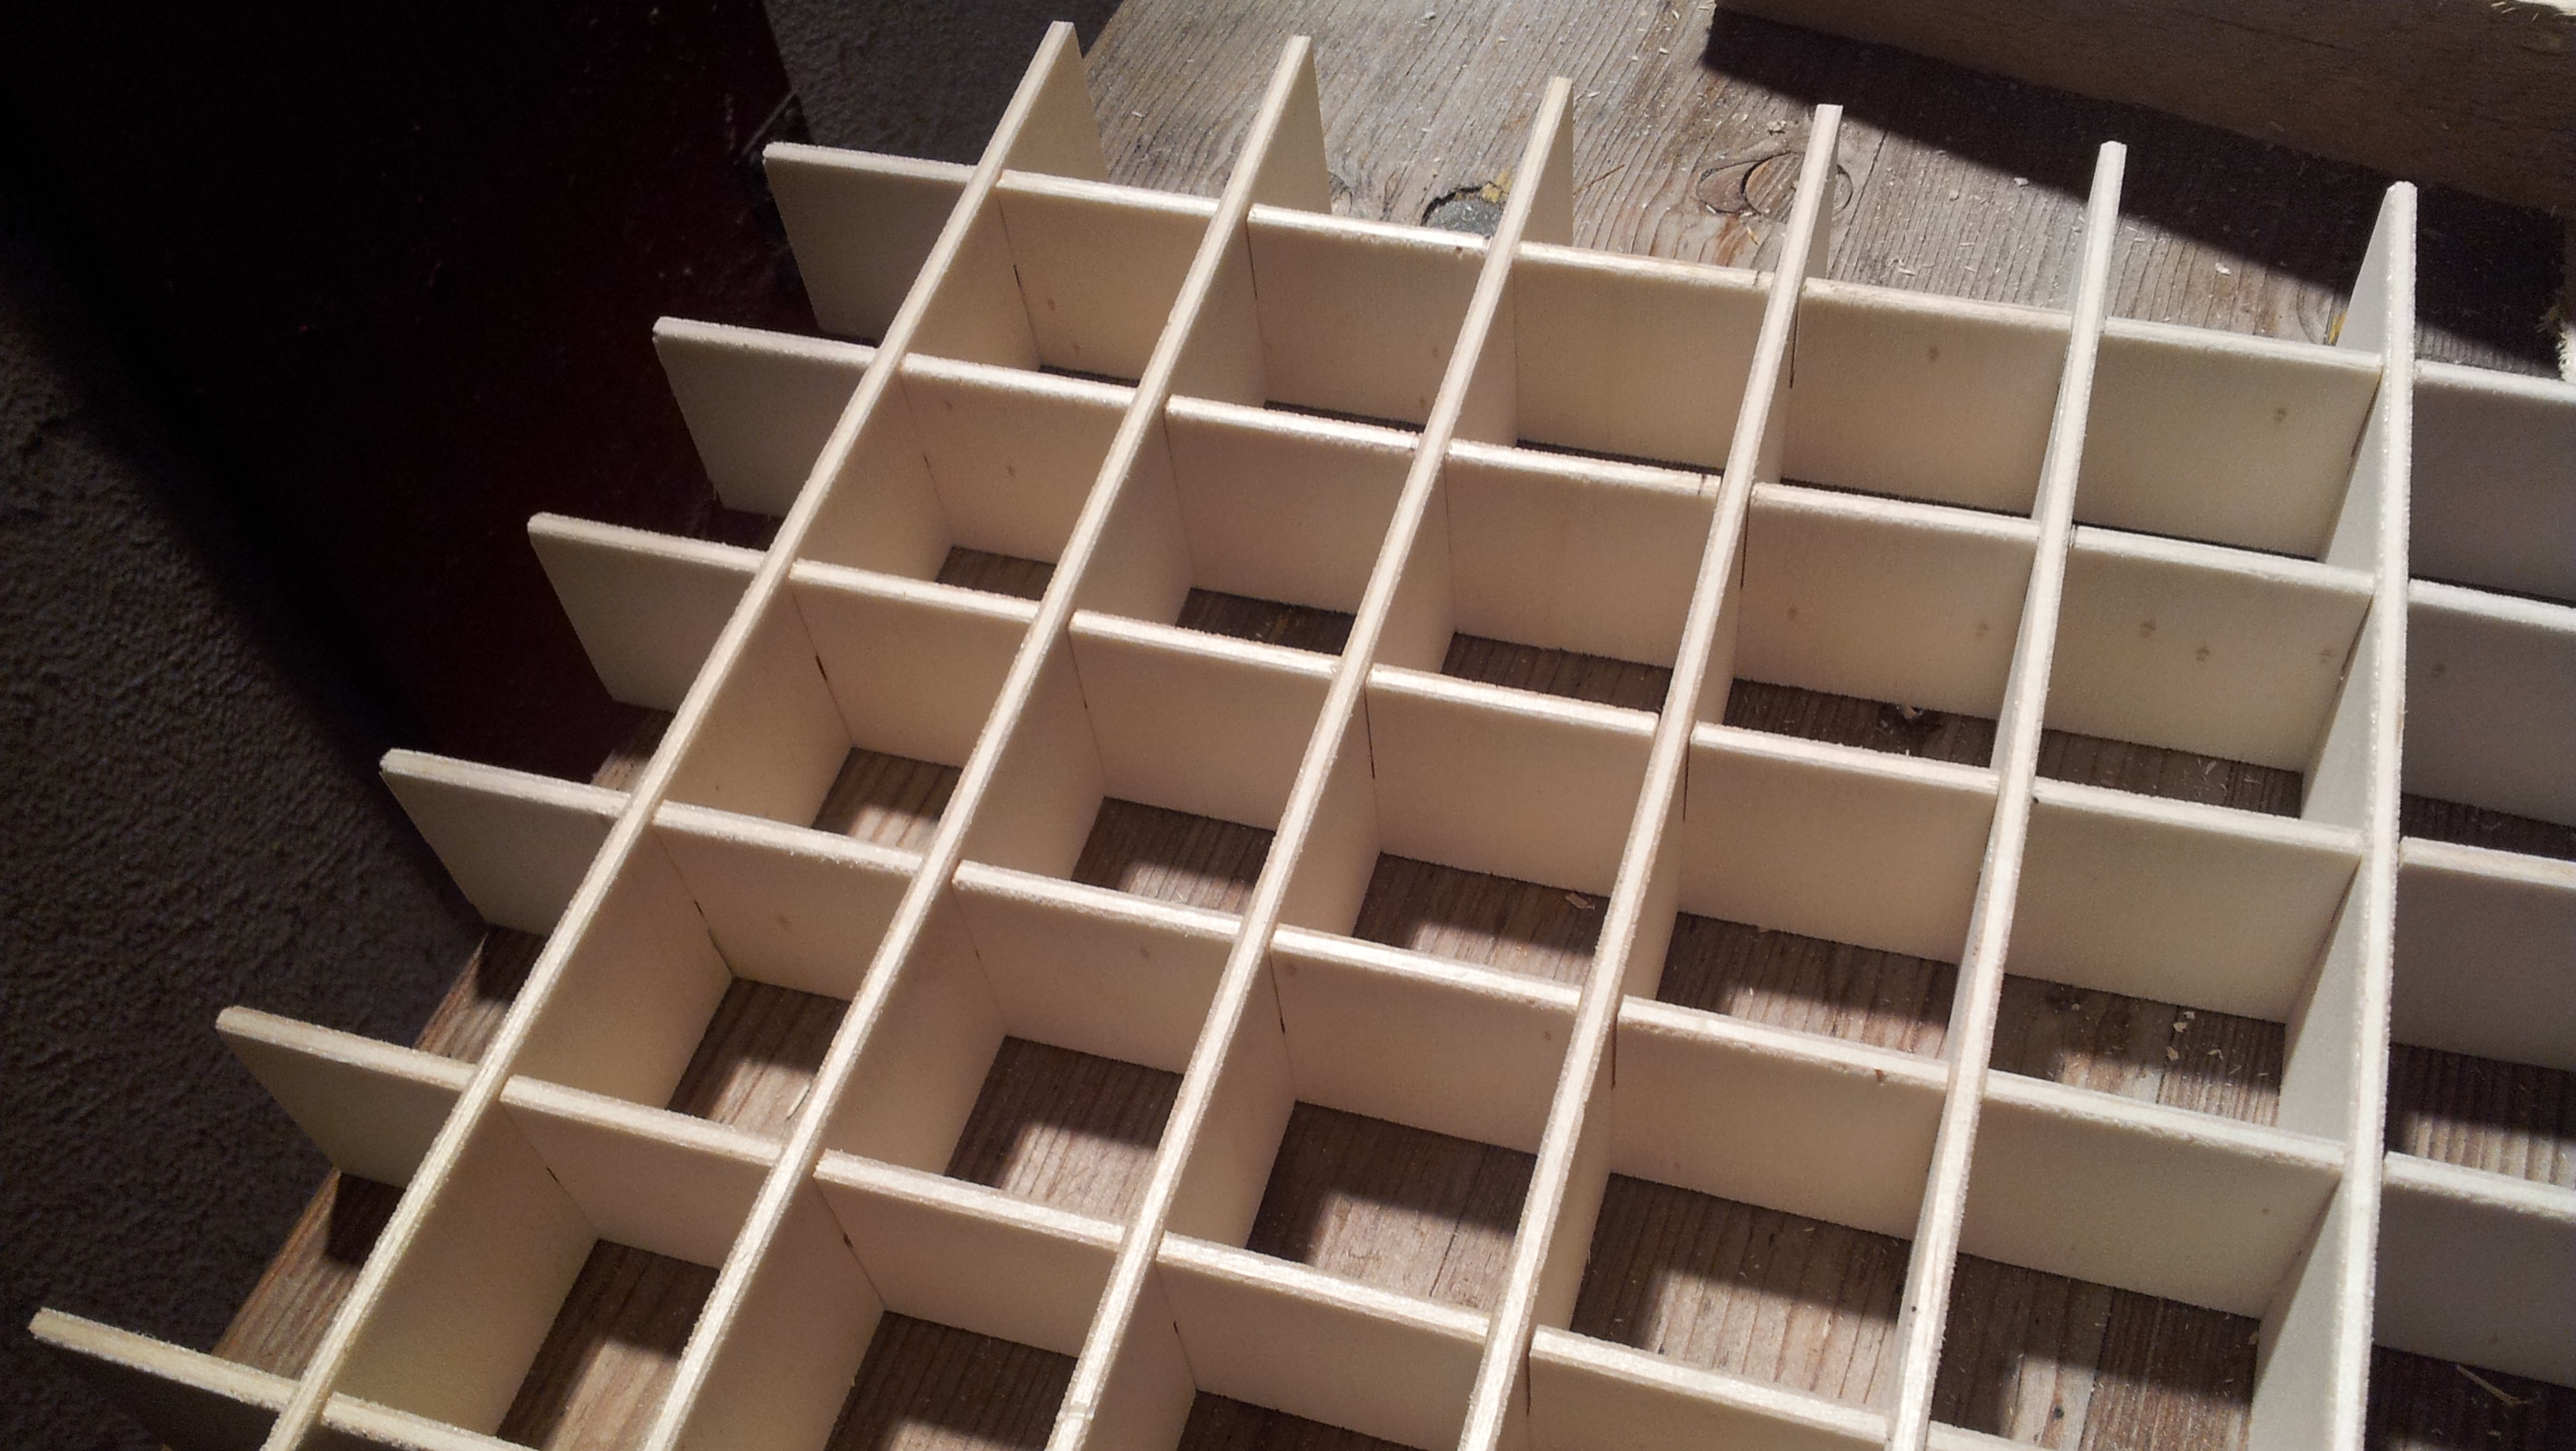
\includegraphics[width=\linewidth]{images/gehaeuse1.jpg}}
\captionof{figure}{Holzgitter für die LED Matrix, gefertigt aus 4mm dickem Sperrholz}\label{fig_gehaeuse1}
\vfill
\centerline{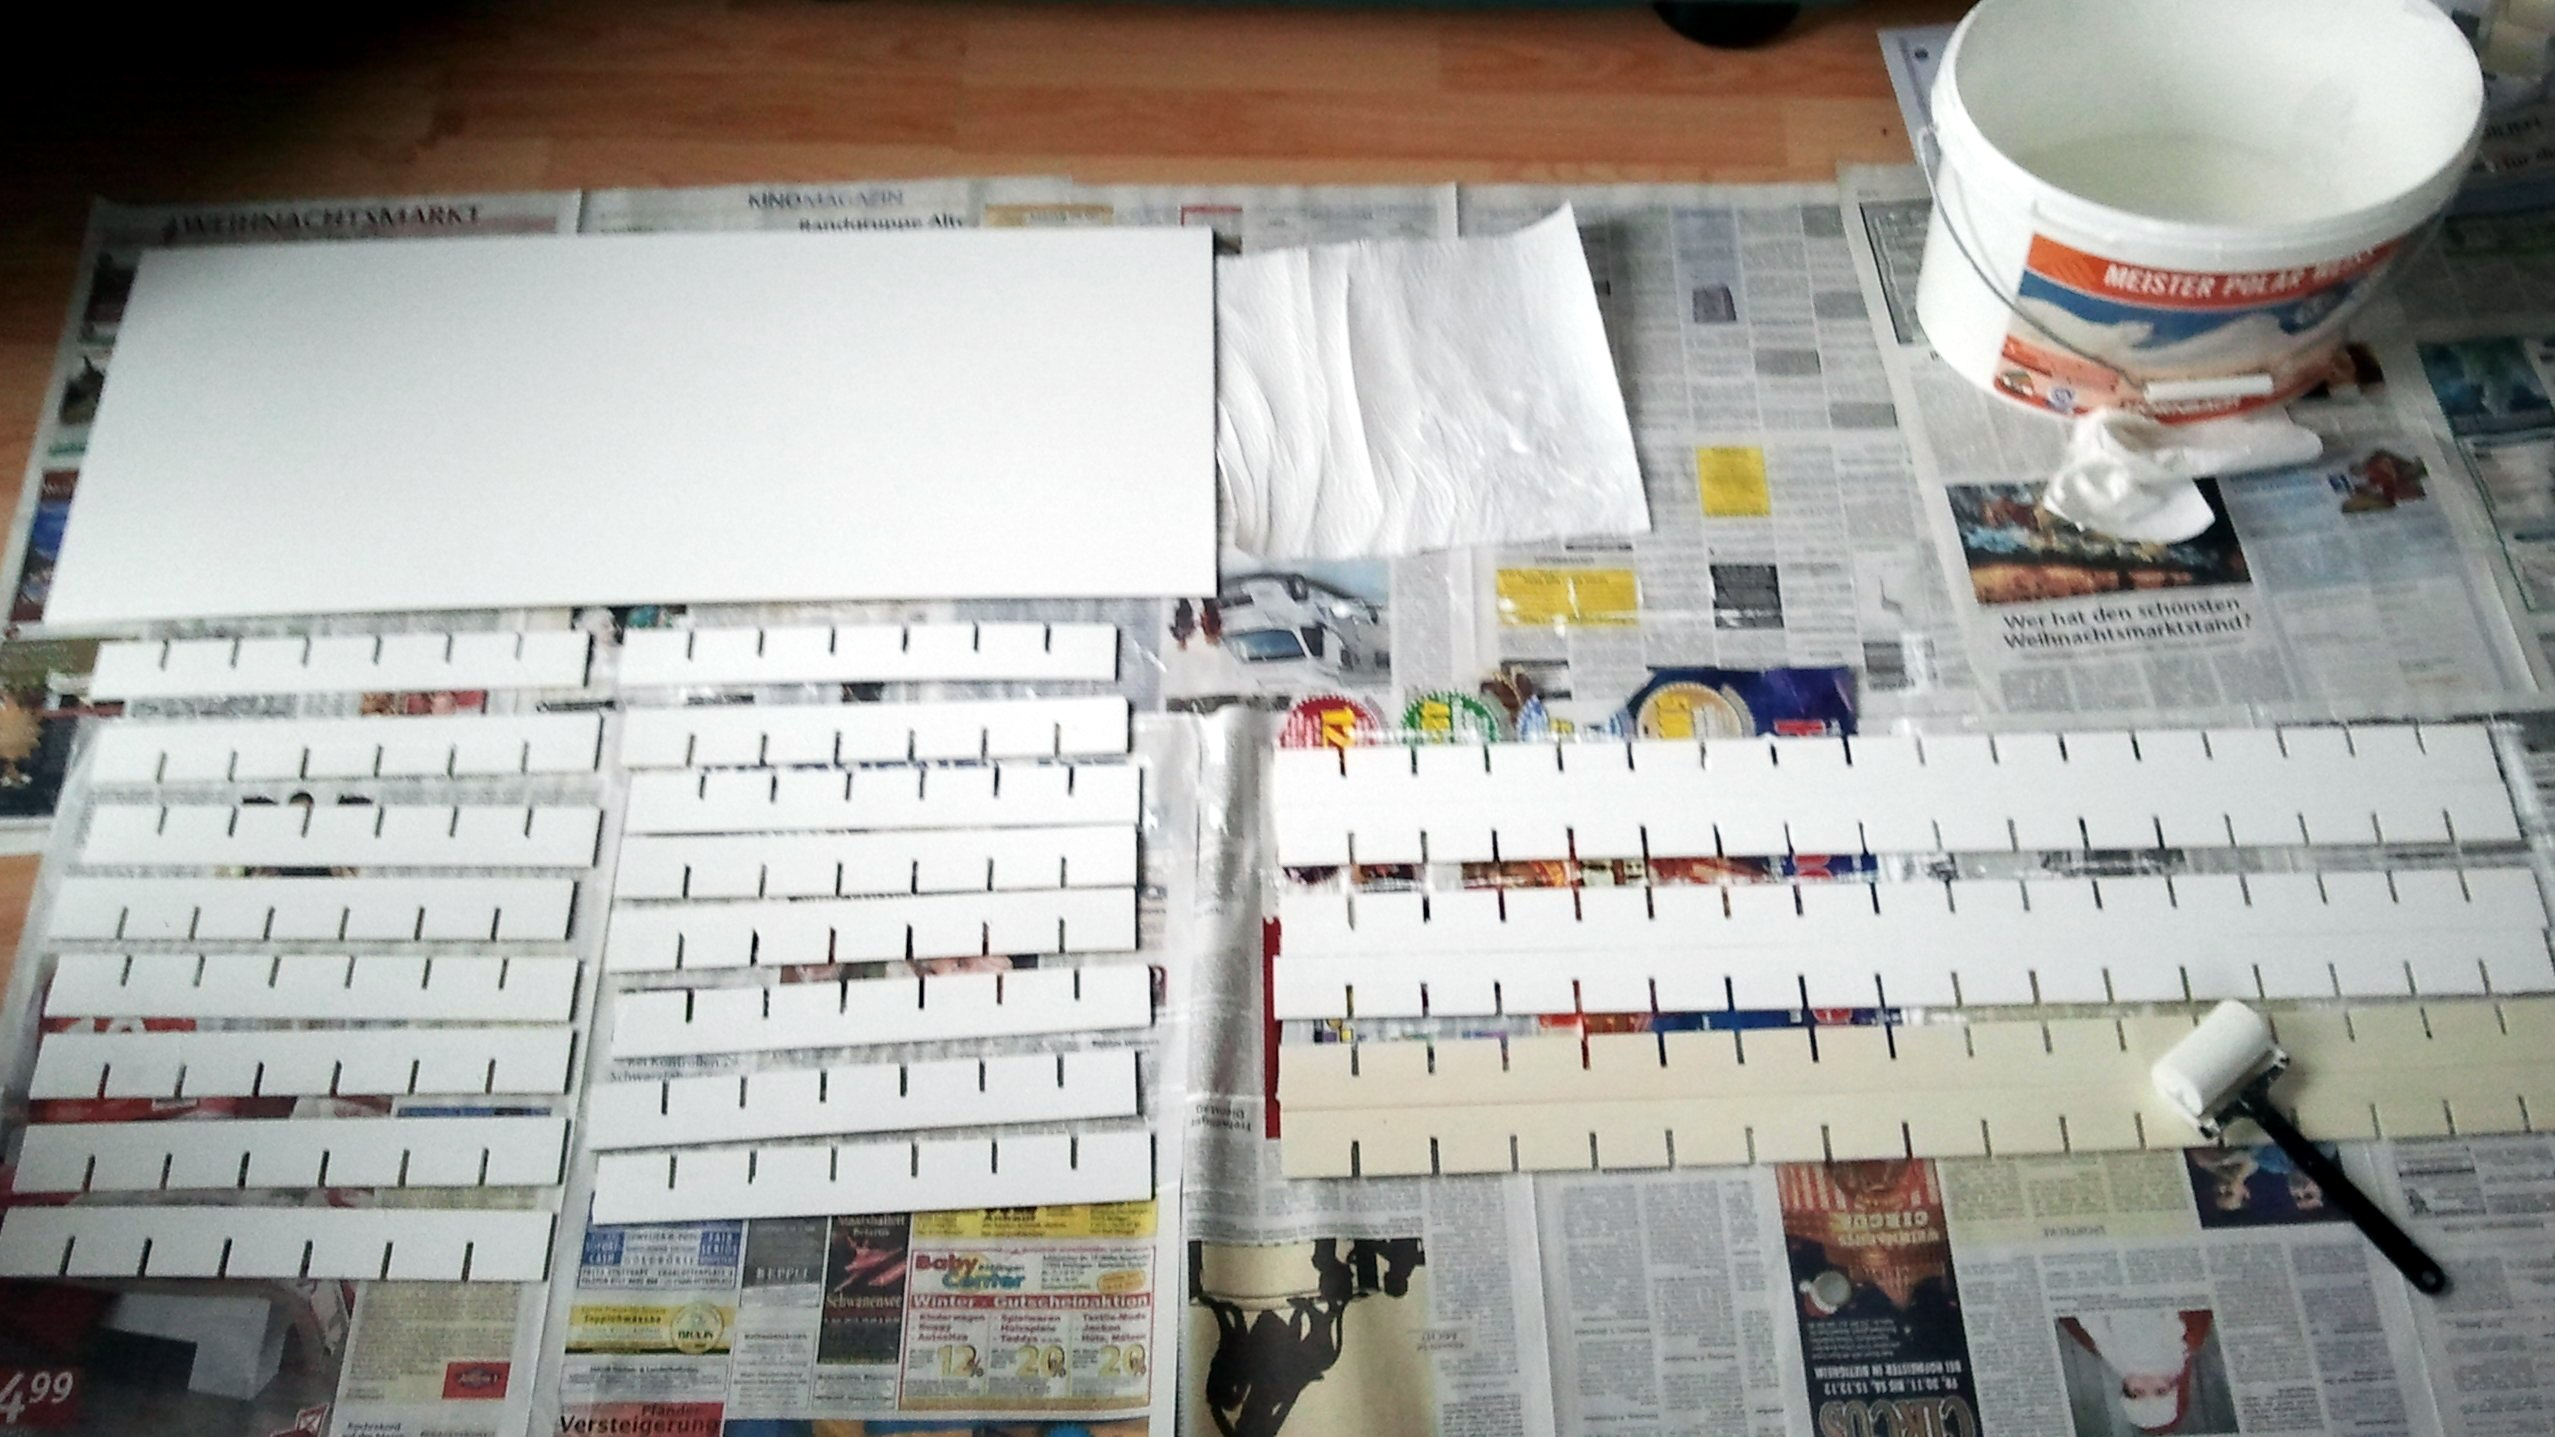
\includegraphics[width=\linewidth]{images/gehaeuse2.jpg}}
\captionof{figure}{Streichen der einzelnen Elemente des Gehäuses}\label{fig_gehaeuse2}
%
\newpage
\centerline{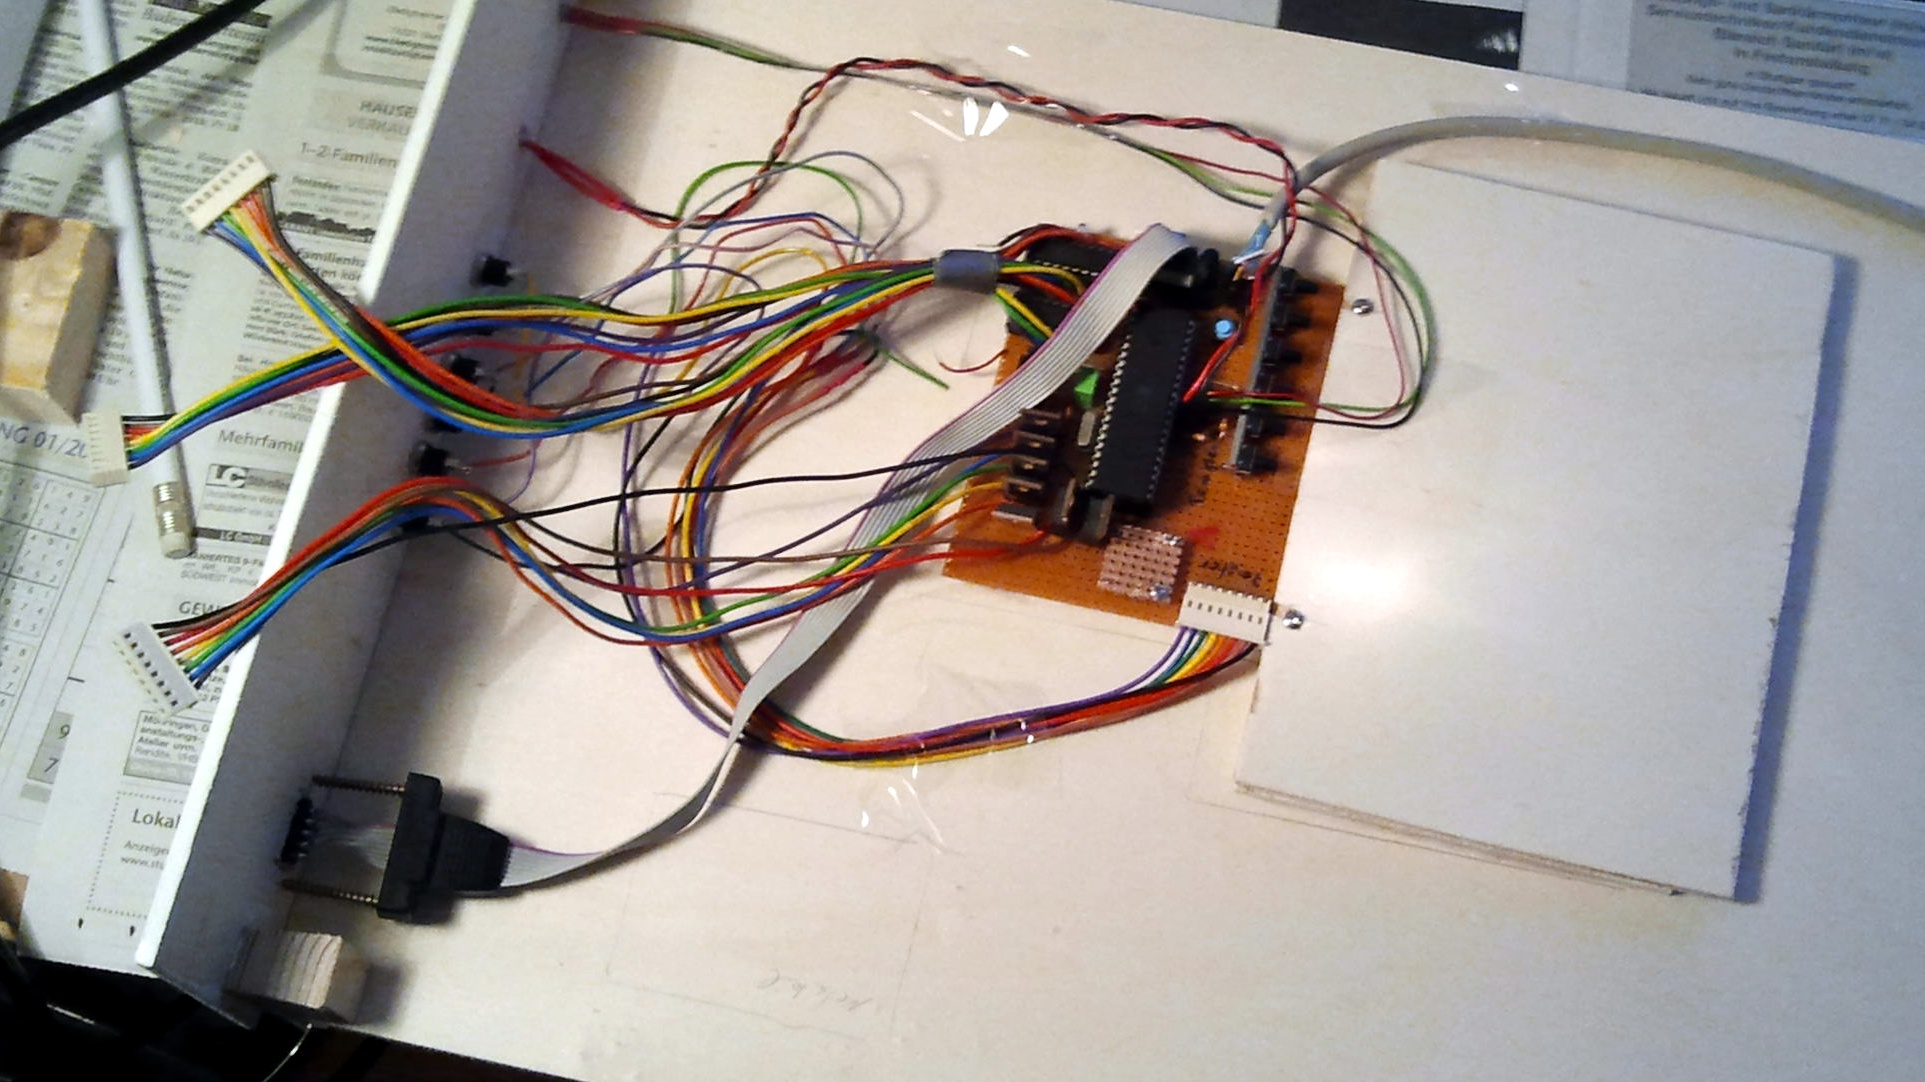
\includegraphics[width=\linewidth]{images/gehaeuse3.jpg}}
\captionof{figure}{Was geht ab}\label{fig_gehaeuse3}
\vfill
\centerline{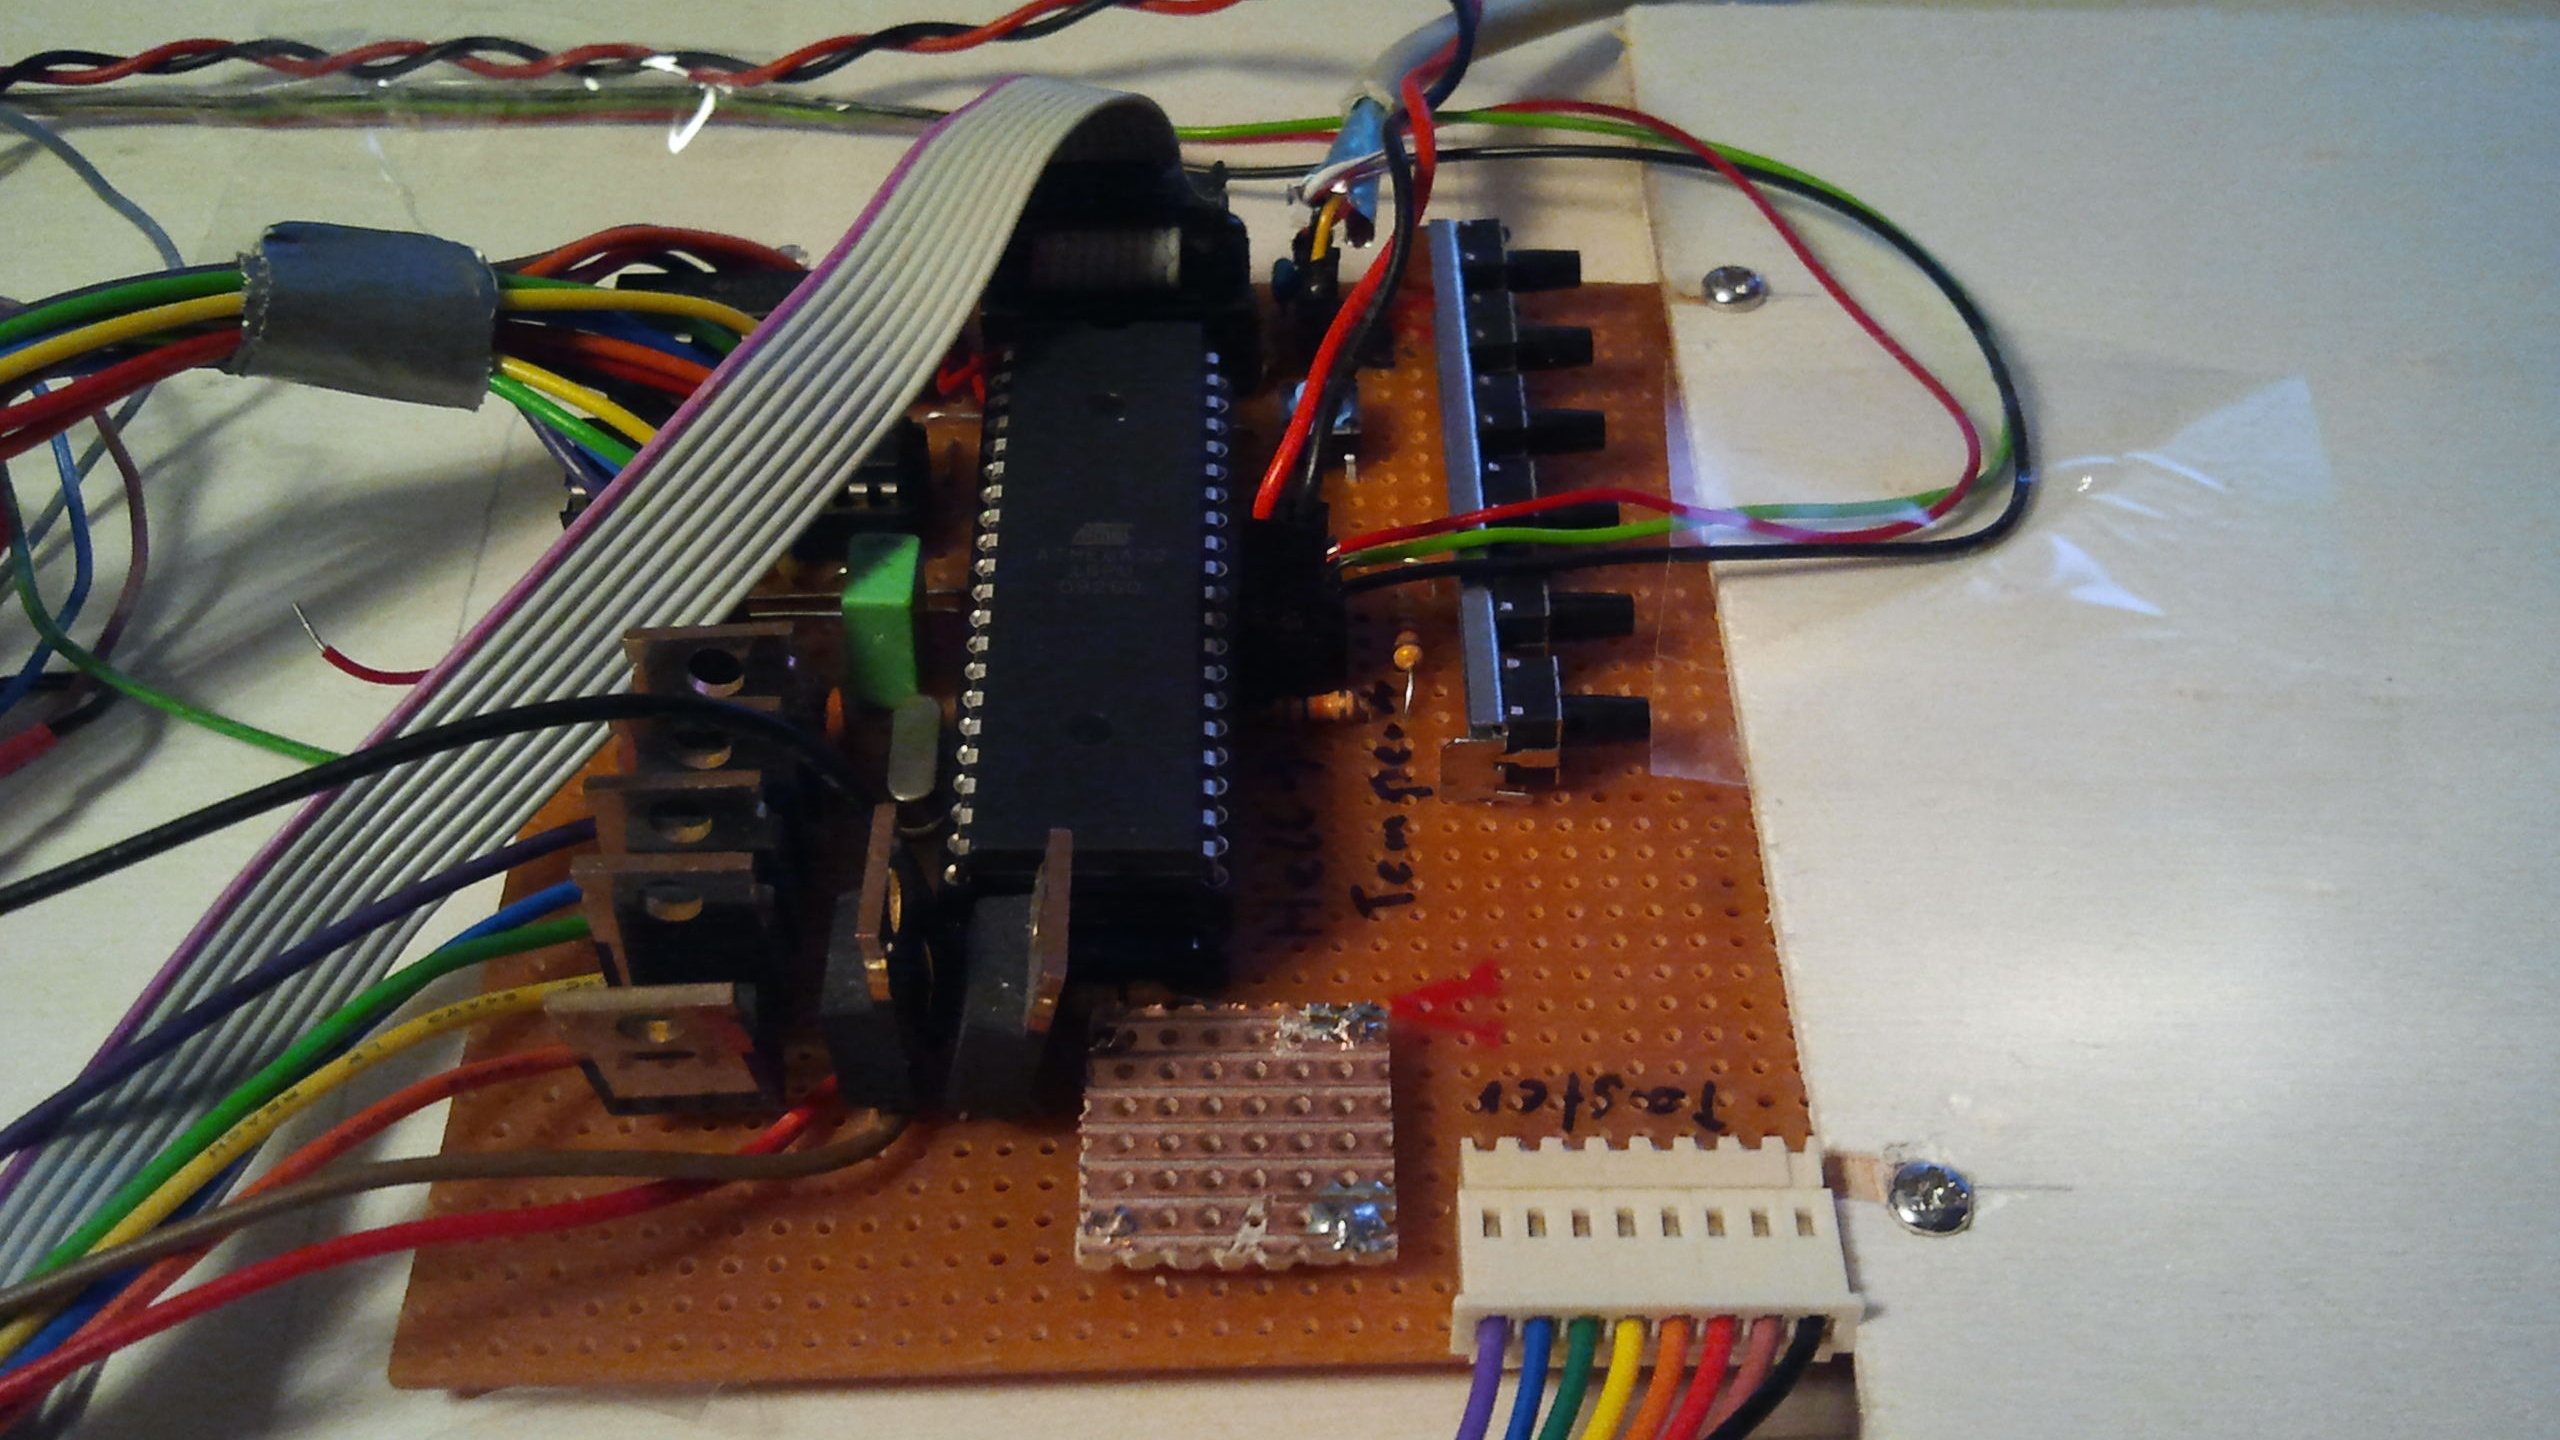
\includegraphics[width=\linewidth]{images/gehaeuse4.jpg}}
\captionof{figure}{Was geht ab}\label{fig_gehaeuse4}
%
\newpage
\centerline{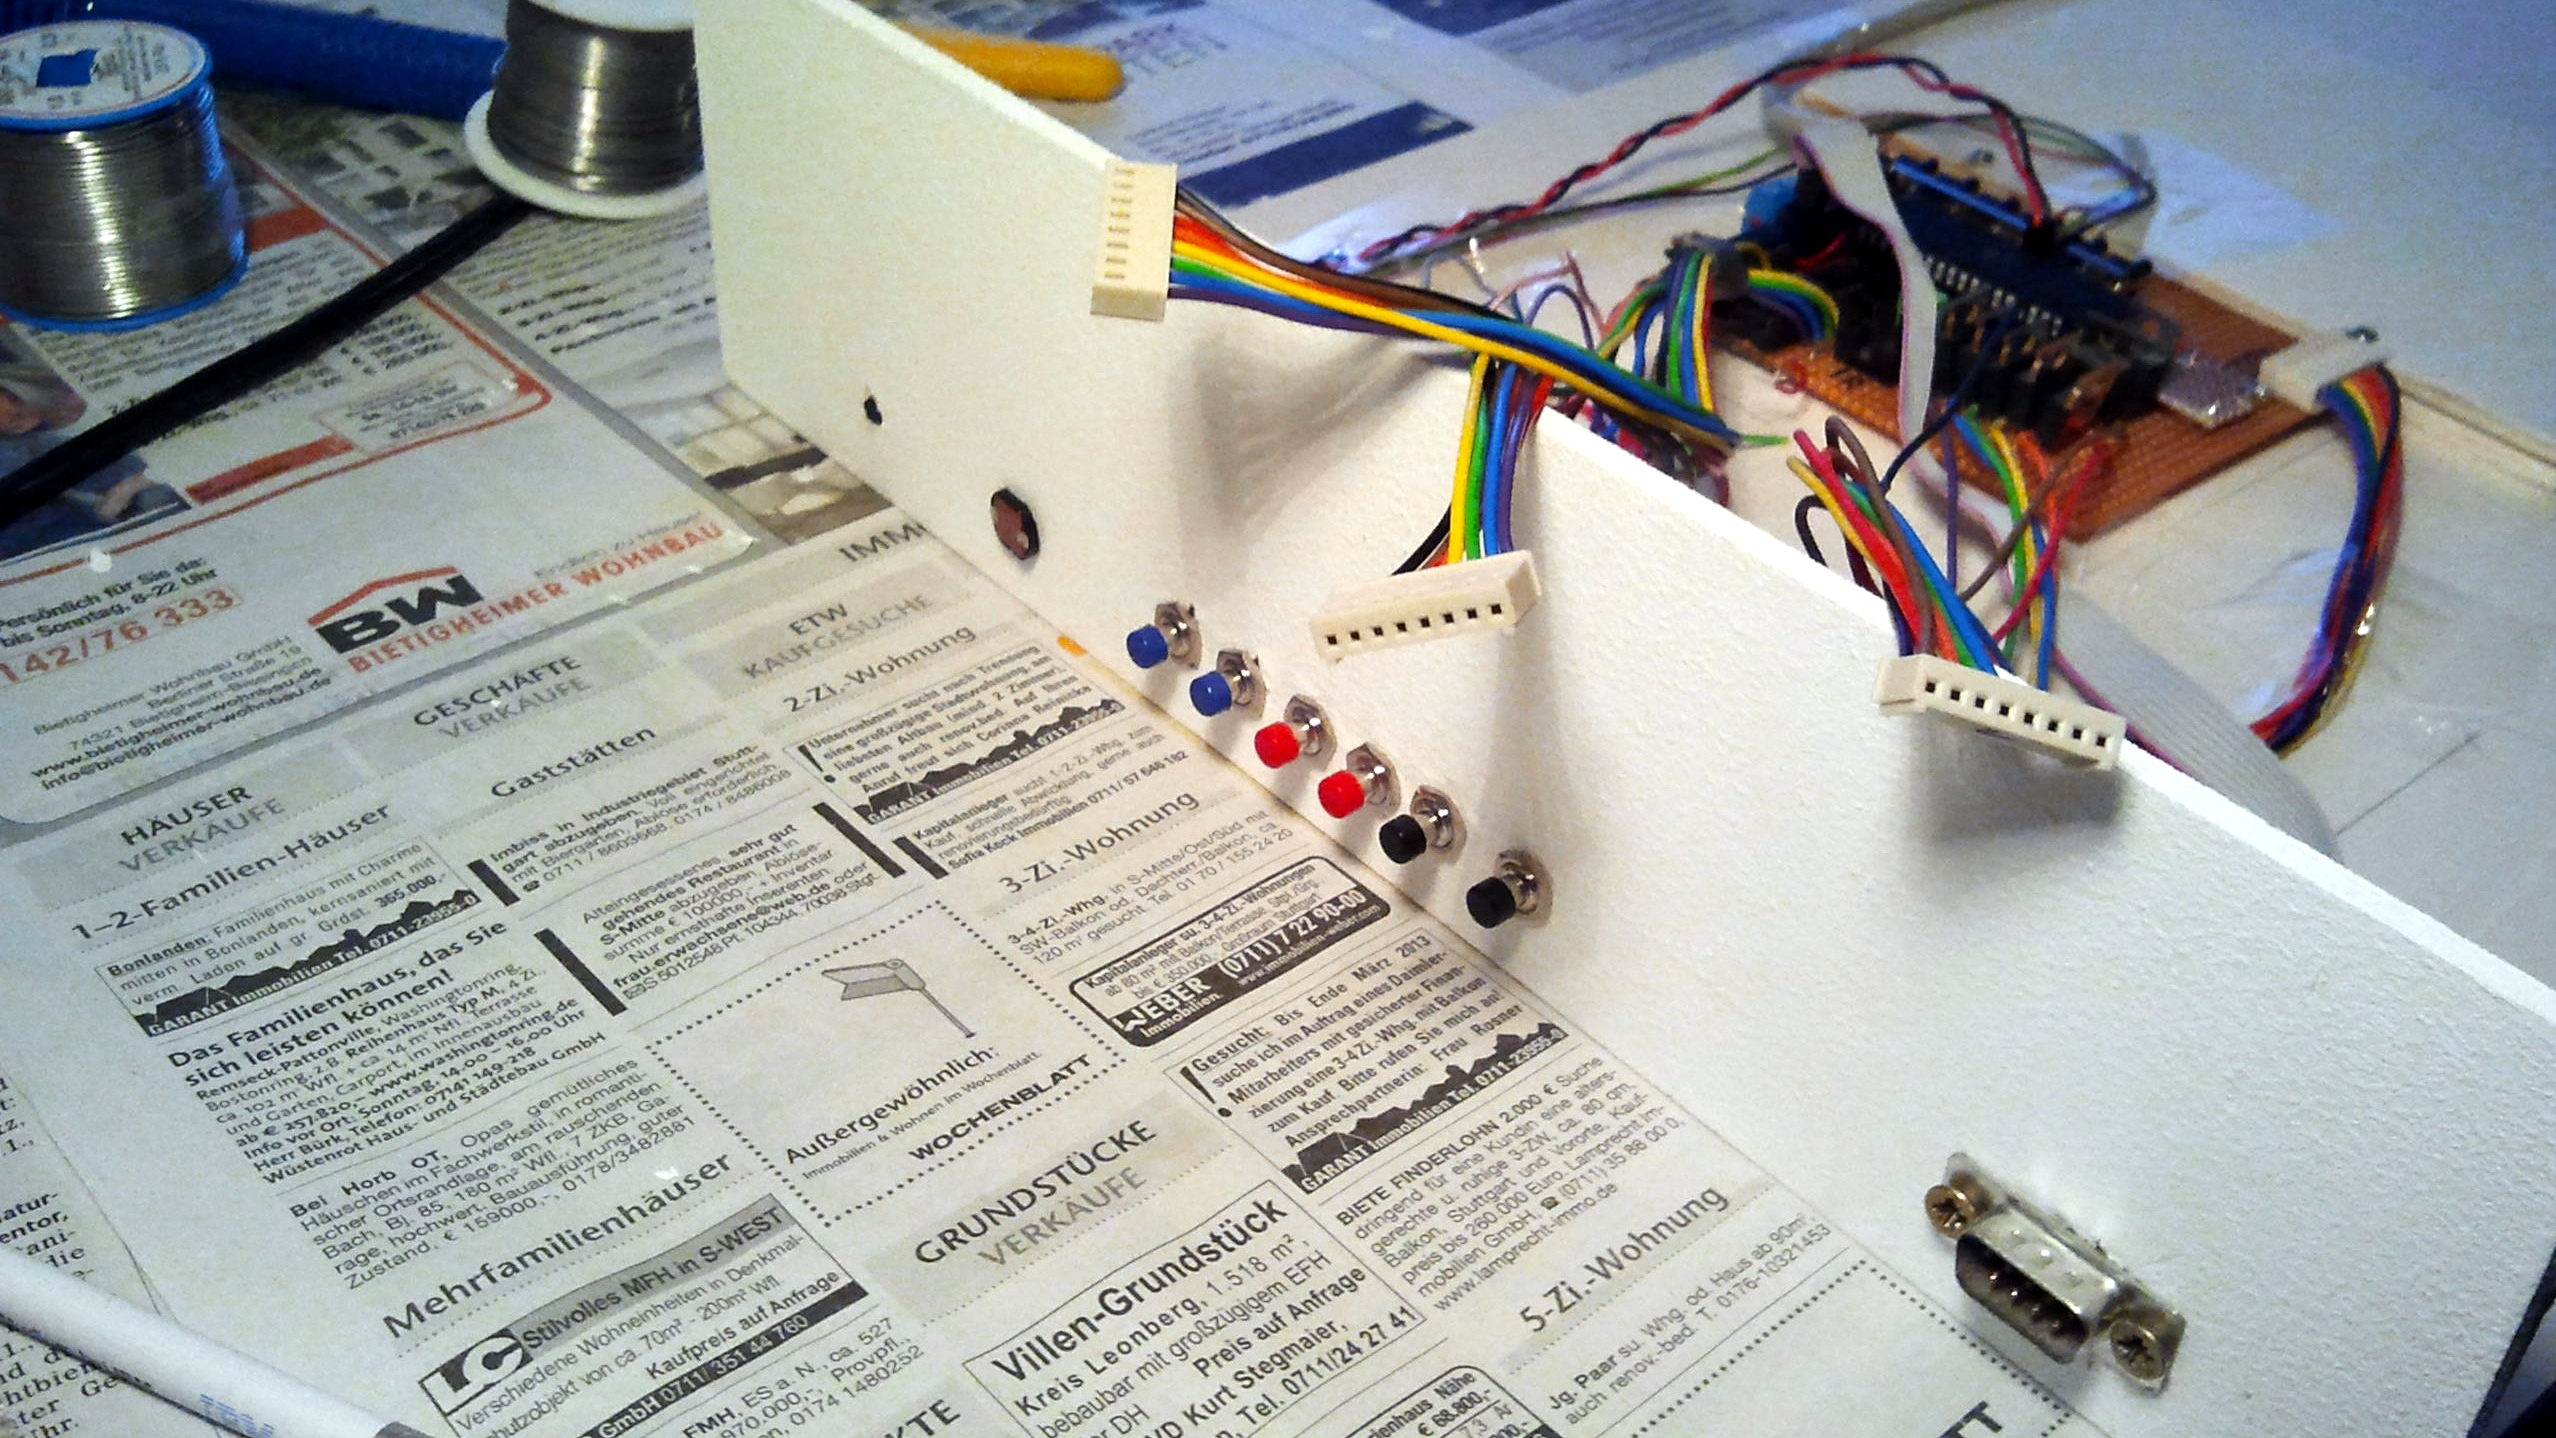
\includegraphics[width=\linewidth]{images/gehaeuse5.jpg}}
\captionof{figure}{Was geht ab}\label{fig_gehaeuse5}
\vfill
\centerline{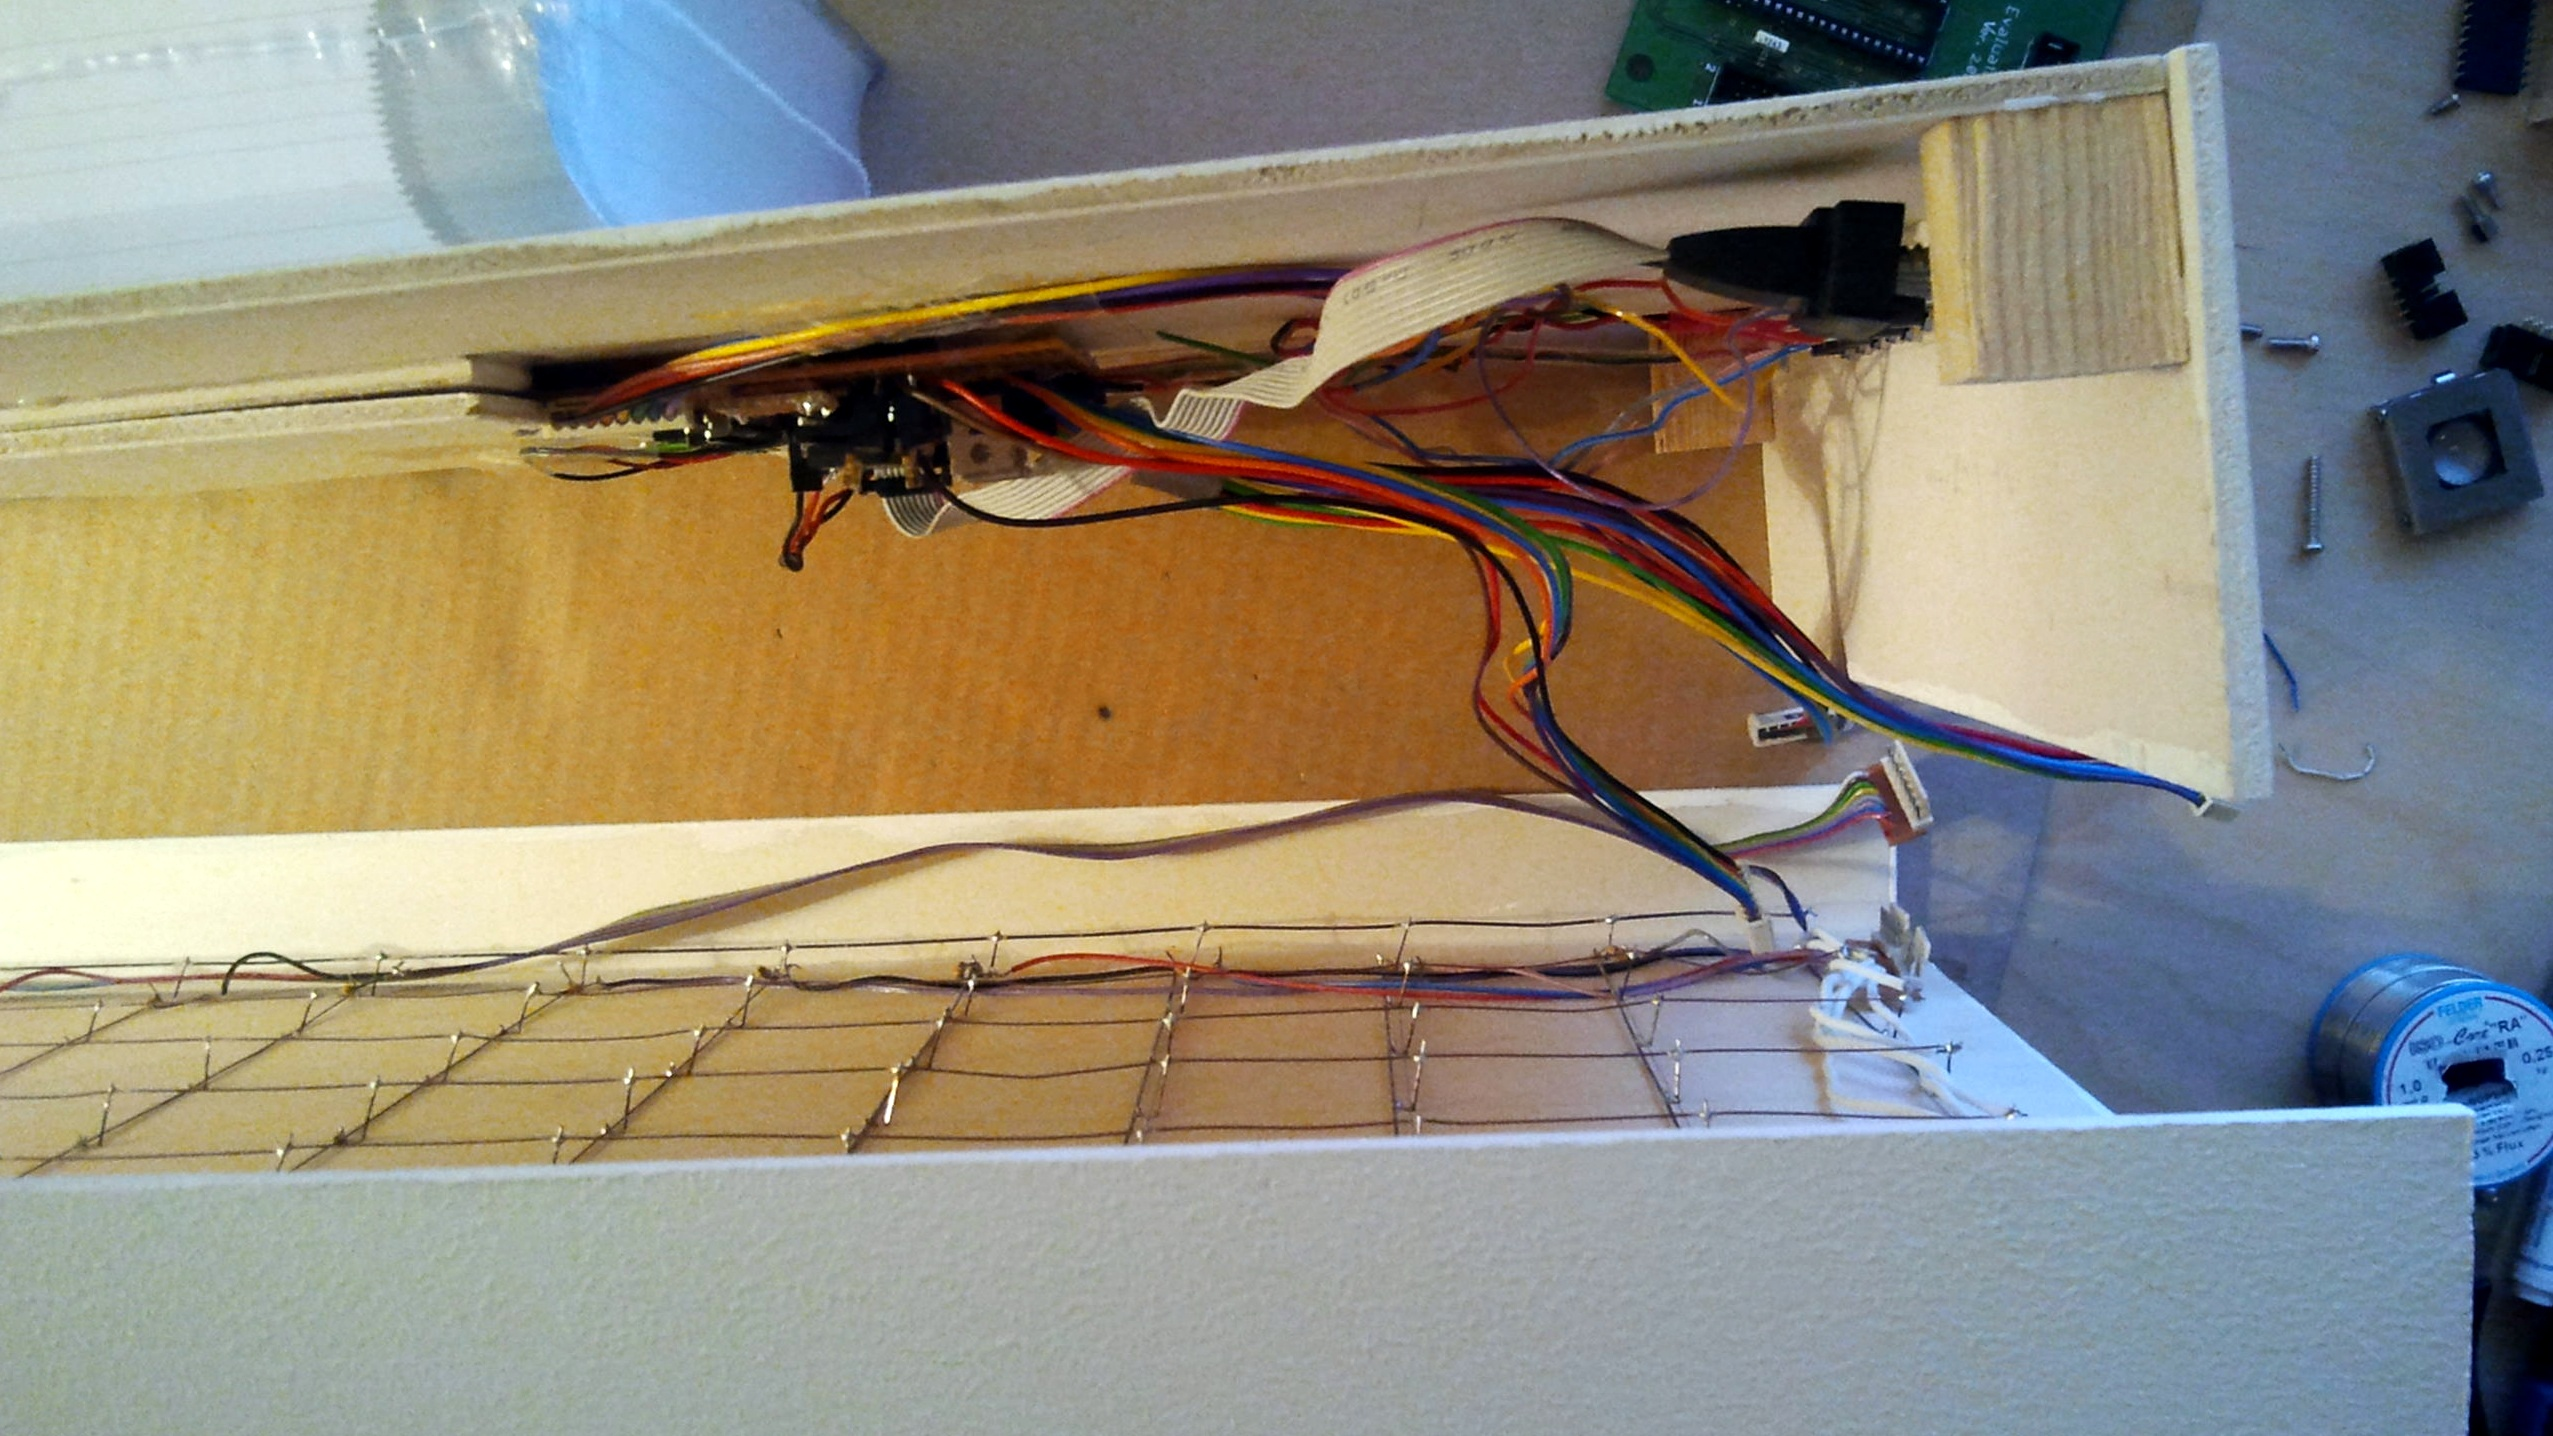
\includegraphics[width=\linewidth]{images/gehaeuse6.jpg}}
\captionof{figure}{Was geht ab}\label{fig_gehaeuse6}
%
\newpage
\centerline{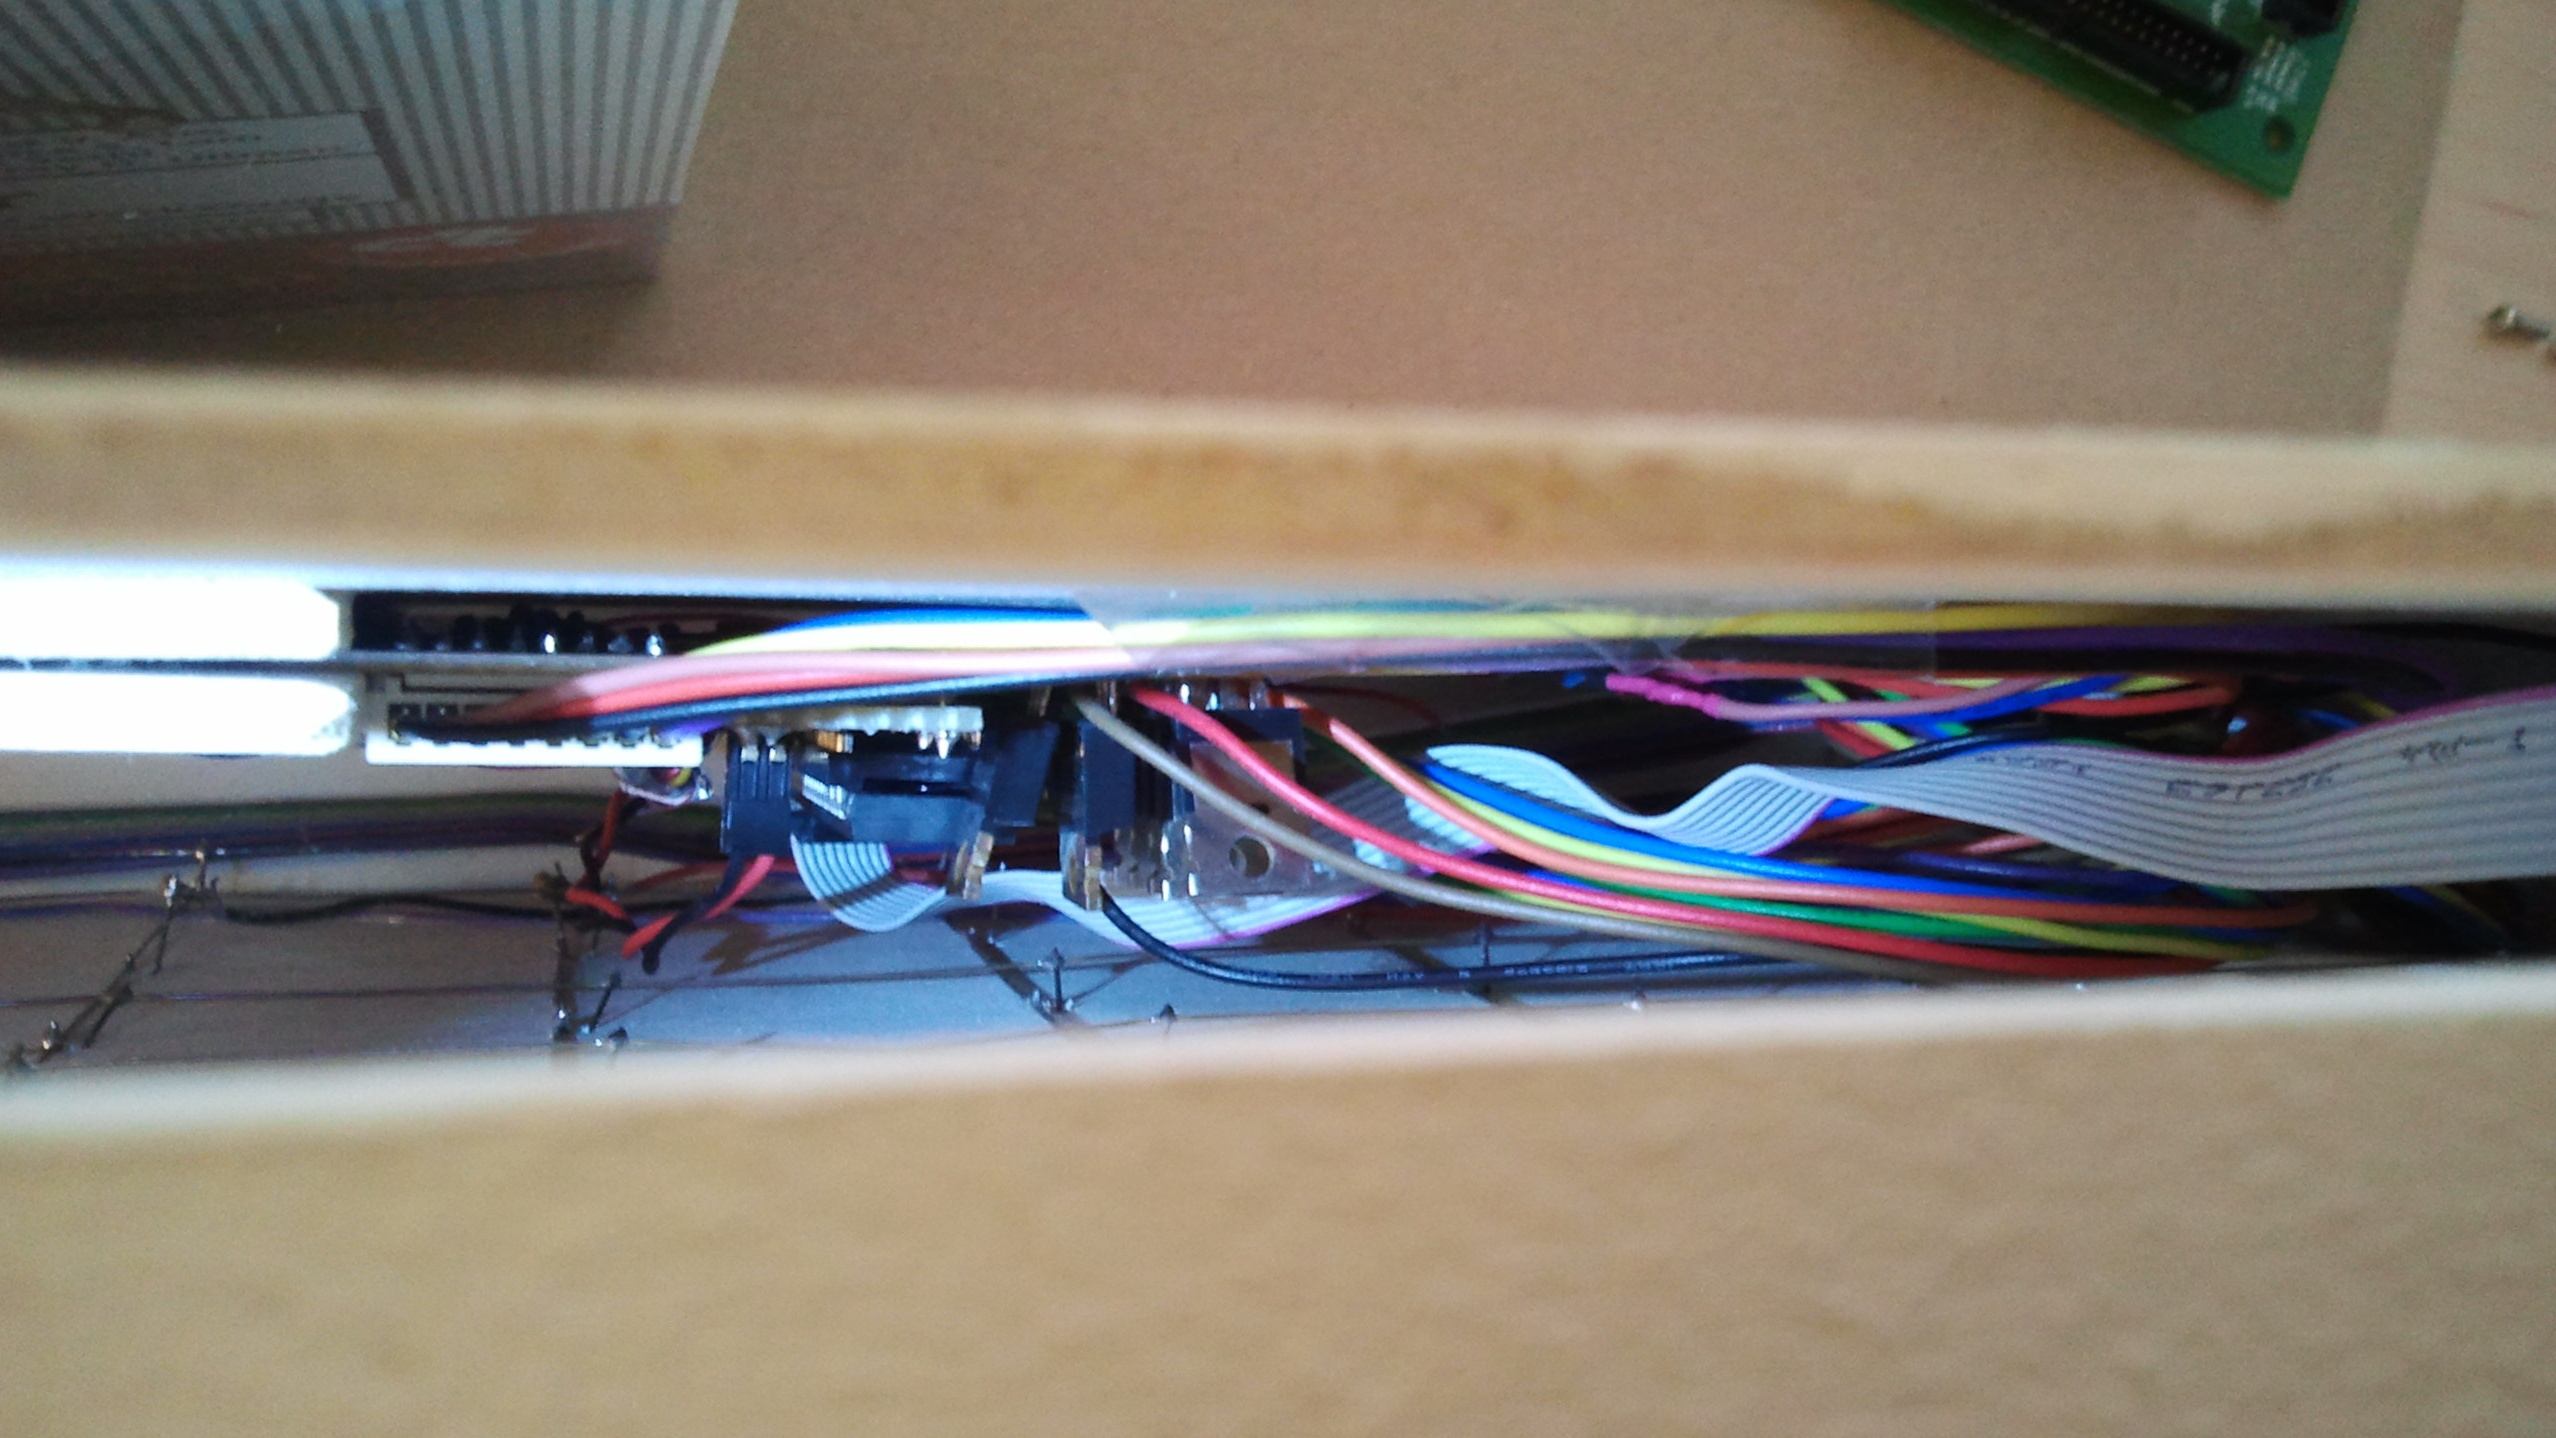
\includegraphics[width=\linewidth]{images/gehaeuse7.jpg}}
\captionof{figure}{Was geht ab}\label{fig_gehaeuse7}
\vfill
\centerline{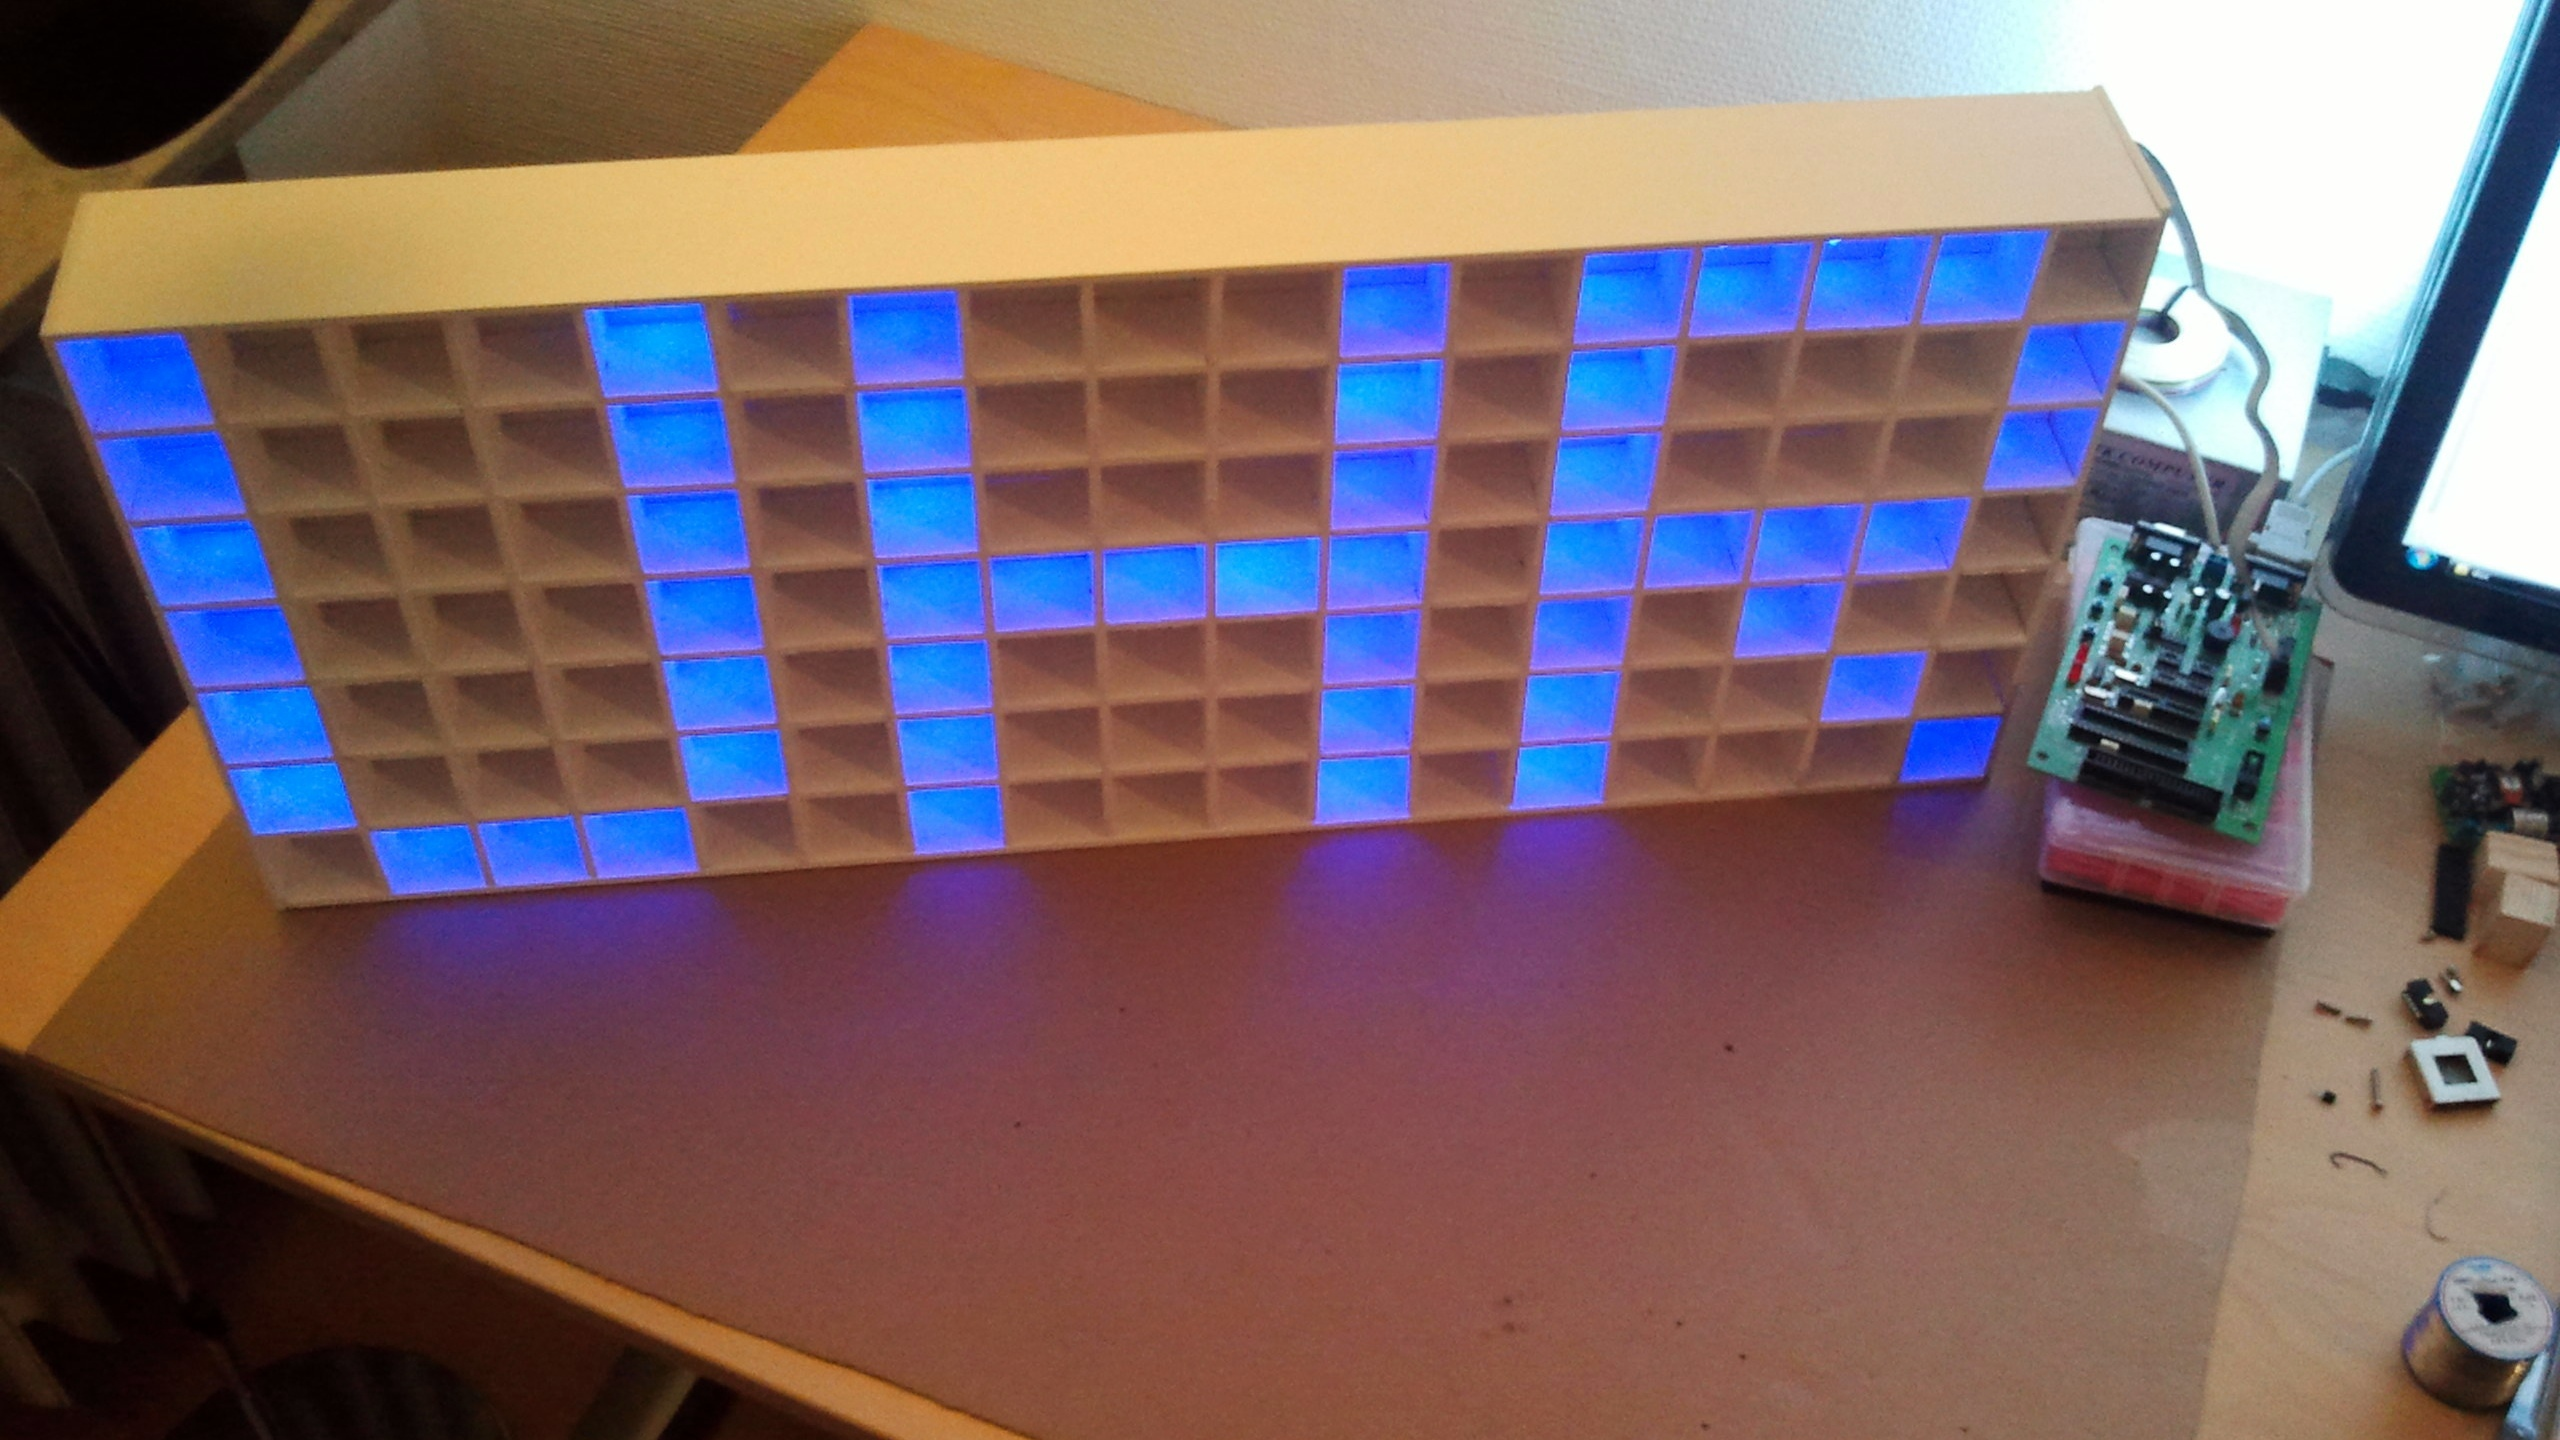
\includegraphics[width=\linewidth]{images/gehaeuse8.jpg}}
\captionof{figure}{Was geht ab}\label{fig_gehaeuse8}
%
\newpage
\section{Quellcode}
TODO